\graphicspath{{Others/}}

\section{Déroulement du projet}
\subsection{Organisation du travail}
\subsubsection{Répartition des tâches et prévision de l'emploi du temps}
Le projet fut dès le départ pensé dans le but d'être simple à séparer sous formes de modules, permettant de travailler en parallèle sur plusieurs fonctionnalités.
Nous avons ensuite estimé le temps de travail nécessaire pour réaliser chaque tâche. 
Nous avions prévu de travailler 4H par semaine de cours et de ne pas travailler les semaines de vacances.
Nous sommes donc arrivé avec l'emploi du temps prévisionnel suivant :
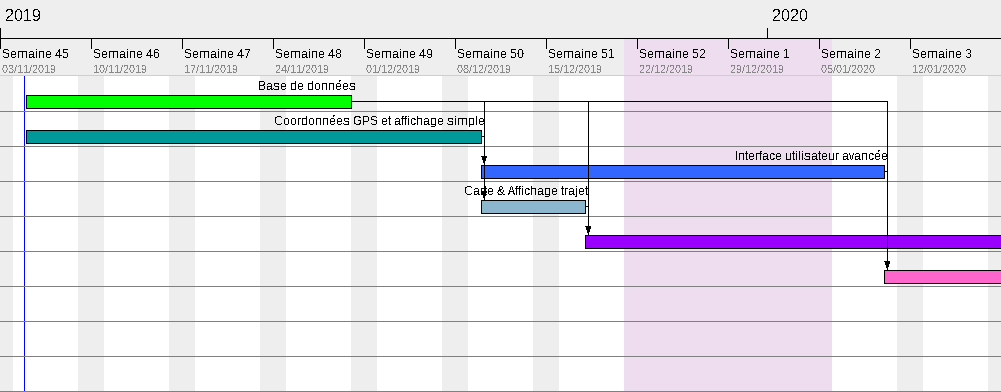
\includegraphics[width=\columnwidth]{test-1.png}
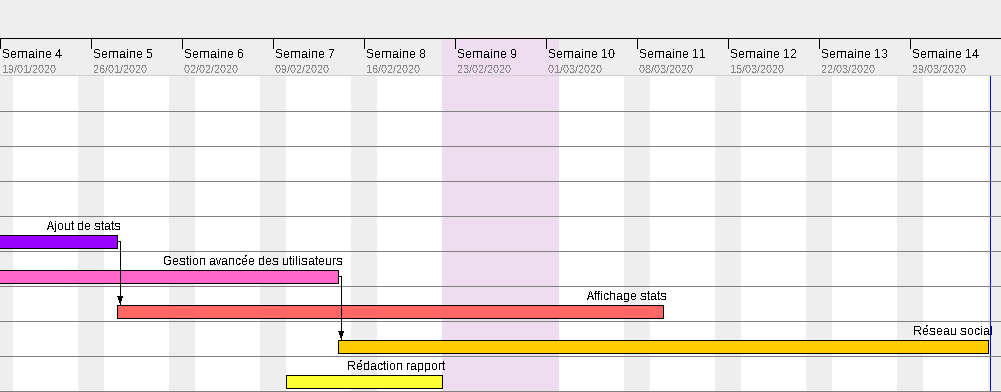
\includegraphics[width=\columnwidth]{test-2.png}
\subsubsection{Problèmes rencontrés et organisation réelle}